\chapter{REST API Proxy \\
  \small{\textit{-- Author Name}}
  \index{Chapter!rest-api-proxy}
  \label{Chapter::RestApiProxy}}

\section{Forwarding API Requests}
When a REST API request is made to OpenTogetherTube, the request is first received by the load balancer. The 
load balancer then selects one of the OTT monoliths based on the current load balancing algorithm, and forwards the 
request to the selected monolith's nginx reverse proxy server. The nginx reverse proxy server receives the request and 
forwards it to the corresponding monolith for processing. 
The monolith processes the request and sends a response back to its nginx reverse proxy server. The reverse proxy server 
then returns the response to the load balancer, which in turn sends the response back to the client that made the original
request.

\begin{figure}[!htb]
  \centering
  \scalebox{0.57}{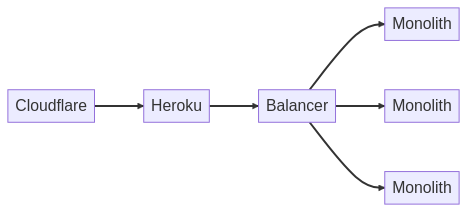
\includegraphics{Figures/api-balancer.png}}
  \caption{\label{Figure::api-balancer} Unloaded Room Sequence Diagram.}
\end{figure}

\section{Forwarding Requests Credentials}

OpenTogetherTube platform uses JSON Web Tokens to authenticate and authorize users. When a user logs in, the 
server generates a JWT that is stored in the browser's local storage and included in all subsequent requests made
by the user. The server verifies the JWT to ensure that the user is authenticated and has permission to access the 
requested video stream.